% \documentclass{acmart}
\documentclass{report}
\usepackage{graphicx}
\usepackage[utf8]{inputenc}
\usepackage[T1]{fontenc}
\usepackage{pgfplots}
\usepackage{pgfplotstable} 
\usepackage{titlesec}
\usepackage{lipsum}
\usepackage{authblk}

\titleformat{\chapter}[display]{\normalfont\bfseries}{}{0pt}{\Large}

\renewcommand*\contentsname{Sumário}

\begin{document}

\title{Aprendizado de Máquina: Trabalho Prático 1}
\author{João Mateus de Freitas Veneroso}
\affil{Departamento de Ciência da Computação da Universidade Federal de Minas Gerais}

\maketitle

\tableofcontents

\chapter{Introdução}

O trabalho prático 1 da disciplina Aprendizado de Máquina determina a implementação de uma rede neural
com uma única camada oculta, utilizando a função de ativação logística e a função de perda Cross Entropy.
Este relatório descreve a implementação de uma rede com estas características e os experimentos realizados
na base Mnist. Os experimentos variaram a taxa de aprendizado, a estratégia de convergência e o número de 
neurônios na camada oculta.

\chapter{Algoritmo}

\section{Rede Neural}

A rede neural foi implementada em C++ sem a utilização de bibliotecas além da STL. O código comporta redes
de múltiplas camadas, mas para fins de experimentação foi utilizada uma única camada oculta. Todos os
neurônios são lineares e a sua saída pode ser descrita pela seguinte função:

\[ y = \sum w_ix_i + b \]

onde $w_i$ representa o peso atribuído à entrada $x_i$ e $b$ representa o viés (variando para cada neurônio). 
Além disso, o resultado da saída de todos os neurônios é normalizado por meio da função logística:

\[ \phi(y) = \frac{1}{1 + e^{-y}} \]

A entrada dos neurônios da camada é composta pelas unidades de entrada da rede. Nos experimentos
realizados, cada neurônio da camada oculta recebeu 784 entradas com um valor entre 0 e 255. Já as
entradas da camada de saída são os resultados das funções de ativação de todos os neurônios da camada oculta. Nos
experimentos realizados, o número de entradas variou entre 25 e 100, dependendo do número de neurônios na 
camada oculta.

O número de neurônios na camada oculta é variável, já o número de neurônios da camada de saída é sempre igual a 10.
Cada neurônio da camada de saída representa a probabilidade das entradas representarem um dígito de 0 a 9. Por exemplo,
o dígito 3 seria representado pela saída \{ 0, 0, 0, 1, 0, 0, 0, 0, 0, 0 \}. Dessa forma, para dado conjunto 
de entradas, a rede utiliza o critério de máxima probabilidade nos neurônios de saída para realizar a previsão final.

\section{Treinamento}

O treinamento da rede foi realizado por meio do algoritmo Backpropagation, utilizando várias estratégias de 
otimização. A função de perda minimizada é chamada de Cross Entropy, cuja definição é:

\[ L(\hat{y}, y) = \frac{1}{m} \sum_{i = 1}^{m} \sum_{k = 1}^{K} -\hat{y}_k^{(i)} log(y_k^{(i)}) -(1 - \hat{y}_k^{(i)}) log(1 - y_k^{(i)}) \]

Onde $ m $ é o número de casos de treino (5000), $ K $ é o número de neurônios de saída (10), $ \hat{y}_k^{(i)} $ é a saída
esperada para o neurônio $ k $ no caso de treino $ i $ e $ y_k^{(i)} $ é a saída do neurônio $ k $ no caso de treino $ i $.
O algoritmo Backpropagation utiliza o gradiente da função de perda para realizar a atualização dos pesos dos neurônios na
direção de maior redução da função de perda. Assim sendo, uma propriedade da derivada da função Cross Entropy entra
em evidência. A derivada da Cross Entropy em relação à saída do neurônio k é:

\[ \frac{\partial L(\hat{y}, y) }{\partial y_k} = \frac{y - \hat{y}}{y(1 - y)} \]

Sabendo que a derivada da função logística é:

\[ \frac{dy}{d[WX + b]} = y(1 - y) \]

podemos cancelar o denominador da derivada parcial da Cross Entropy no cálculo de atualização dos pesos da camada de saída, o que torna o cálculo 
dos novos pesos trivial. Já a propagação do gradiente para a camada oculta prossegue como faríamos com qualquer outra 
função de perda.

\section{Estratégias de Otimização}

Os experimentos consideraram quatro formas distintas de otimização dos pesos, que se diferenciaram pela frequência
de atualização dos pesos dentro de uma época (5000 casos de treinamento). Para melhorar 
a taxa de convergência é possível utilizar as técnicas de Momentum e Weight Decay, no entanto, os experimentos
foram realizados sem a utilização destas técnicas.

\subsection{Gradient Descent (GD)}

A atualização dos pesos só ocorre no final de cada época, sendo que o gradiente dos pesos é aprimorado a cada caso de treinamento. 
Esta estratégia garante que a direção de atualização dos pesos será ótima para reduzir a função de perda naquele conjunto de 
de treinamento, no entanto, a frequência de atualização é muito baixa (1 vez a cada 5000 casos) o que pode resultar em uma taxa
baixa de convergência.

\subsection{Stochastic Gradient Descent (SGD)}

A atualização dos pesos ocorre ao final de cada caso de treinamento. O gradiente pode se comportar de forma errática, mas a frequência
de atualização é 5000 vezes mais alta do que no Gradient Descent (1 vez a cada caso de treinamento).

\subsection{Mini Batch 10}

É uma estratégia intermediária entre o Gradient Descent e o Stochastic Gradient Descent. Os pesos são atualizados a cada 10
casos de treinamento.

\subsection{Mini Batch 50}

Igual ao Mini Batch 10, no entanto, os pesos são atualizados a cada 50 iterações.

\chapter{Experimentos}

Todos os experimentos utilizaram a base Mnist com 5000 casos de treinamento e rodaram por 1000 épocas. Em todos os experimentos,
os pesos dos neurônios foram inicializados de forma aleatória com um valor entre -4 e 4. O número de neurônios
na camada oculta variou entre 25, 50 e 100 e a taxa de aprendizado variou entre 0.5, 1 e 10 para cada uma das quatro
estratégias de otimização descritas anteriormente, o que resultou em 36 experimentos diferentes. A tabela 3.1
descreve o erro empírico mínimo para cada um dos modelos utilizados e o valor da função Cross Entropy no erro mínimo.
$ \eta $ representa a taxa de aprendizado e $ N $ o número de nerônios na camada oculta da rede.
O gráfico de convergência para cada um dos experimentos está descrito nas figuras 3.1 a 3.12.

\begin{table}
\centering
\begin{tabular}{ |l|l|l| l l| }
  \hline
  \multicolumn{5}{|c|}{Erro empírico mínimo por modelo de otimização} \\
  \hline
  Modelo & N & $ \eta $ & Cross Entropy & Erro Empírico \\
  \hline
  GD              & 25   & 0.5 & 1.29037  & 22.4\% \\
  GD              & 25   & 1   & 0.975634 & 16.2\% \\
  GD              & 25   & 10  & 0.538274 & 8.1\%  \\
  \hline
  GD              & 50   & 0.5 & 1.03982  & 15.2\% \\
  GD              & 50   & 1   & 0.730567 & 10.2\% \\
  GD              & 50   & 10  & 0.440681 & 5.7\%  \\
  \hline
  GD              & 100  & 0.5 & 0.769577 & 8.8\%  \\
  GD              & 100  & 1   & 0.426178 & 4.1\%  \\
  GD              & 100  & 10  & 0.28649  & 2.3\%  \\
  \hline
  SGD             & 25  & 0.5  & 0.802409 & 12.3\% \\
  SGD             & 25  & 1    & 0.936852 & 15.1\% \\
  SGD             & 25  & 10   & 4.5451   & 29.5\% \\
  \hline
  SGD             & 50  & 0.5  & 0.707264 & 9.4\% \\
  SGD             & 50  & 1    & 0.878354 & 13.6\% \\
  SGD             & 50  & 10   & 3.35968  & 18.4\% \\
  \hline
  SGD             & 100 & 0.5  & 0.646608 & 7.0\%  \\ 
  SGD             & 100 & 1    & 0.533079 & 5.1\% \\
  SGD             & 100 & 10   & 2.54651  & 15.3\% \\
  \hline
  MINI\_BATCH\_10 & 25  & 0.5 & 0.840565 & 15\%   \\
  MINI\_BATCH\_10 & 25  & 1   & 0.641306 & 9.1\%  \\    
  MINI\_BATCH\_10 & 25  & 10  & 1.31211  & 24\%   \\
  \hline
  MINI\_BATCH\_10 & 50  & 0.5 & 0.406151 & 6\%    \\
  MINI\_BATCH\_10 & 50  & 1   & 0.411477 & 5.4\%  \\
  MINI\_BATCH\_10 & 50  & 10  & 1.15512  & 17.4\% \\
  \hline
  MINI\_BATCH\_10 & 100 & 0.5 & 0.36138  & 5.1\%  \\
  MINI\_BATCH\_10 & 100 & 1   & 0.411884 & 4.9\%  \\
  MINI\_BATCH\_10 & 100 & 10  & 0.500474 & 6.7\%  \\
  \hline
  MINI\_BATCH\_50 & 25  & 0.5 & 0.684446 & 11.1\% \\
  MINI\_BATCH\_50 & 25  & 1   & 0.656606 & 12.2\% \\
  MINI\_BATCH\_50 & 25  & 10  & 1.10615  & 16.9\% \\
  \hline
  MINI\_BATCH\_50 & 50  & 0.5 & 0.50873  & 7\%    \\
  MINI\_BATCH\_50 & 50  & 1   & 0.456375 & 5.2\%  \\
  MINI\_BATCH\_50 & 50  & 10  & 0.482317 & 6.3\%  \\
  \hline
  MINI\_BATCH\_50 & 100 & 0.5 & 0.367179 & 4.1\%  \\
  MINI\_BATCH\_50 & 100 & 1   & 0.420391 & 5.1\%  \\
  MINI\_BATCH\_50 & 100 & 10  & 0.247238 & 2.4\%  \\
  \hline
\end{tabular}
\label{tab:min_error}
\caption{Erro empírico mínimo}
\end{table}

\begin{figure}
  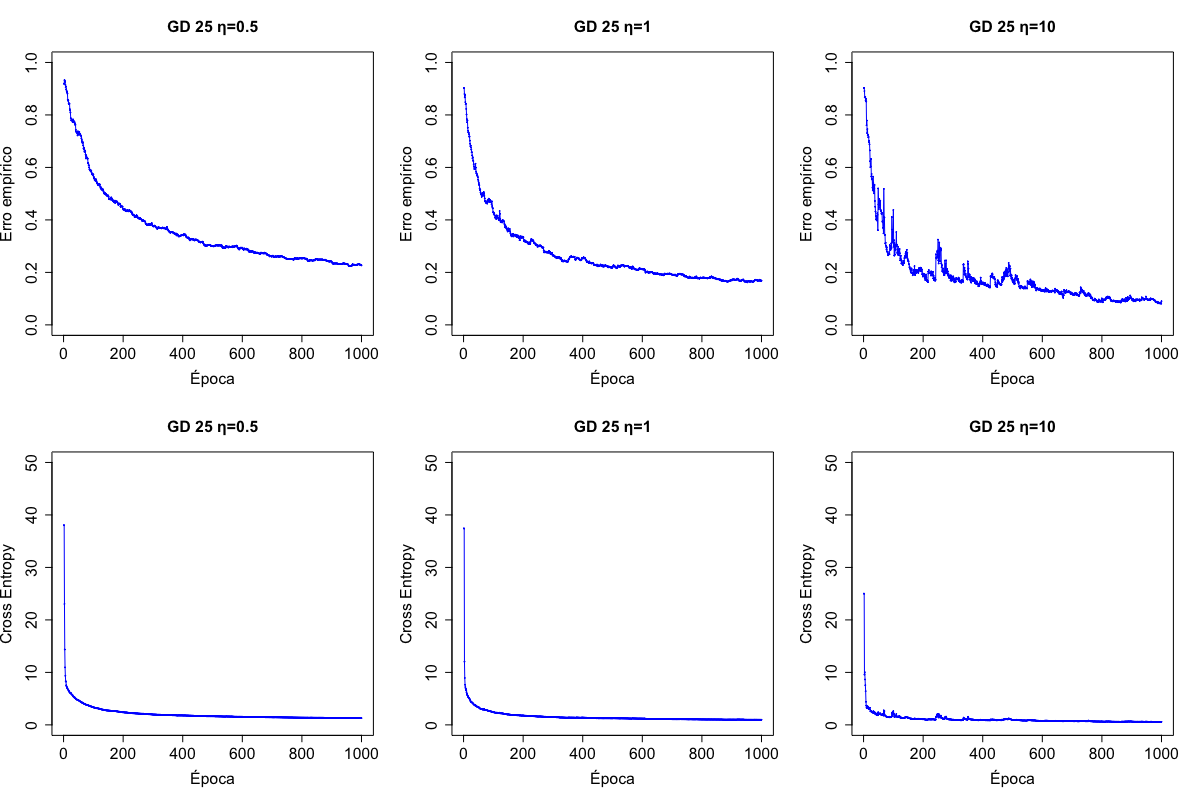
\includegraphics[width=\linewidth]{gd_25.png}
  \label{fig:gd_25}
  \caption{GD 25}
\end{figure}

\begin{figure}
  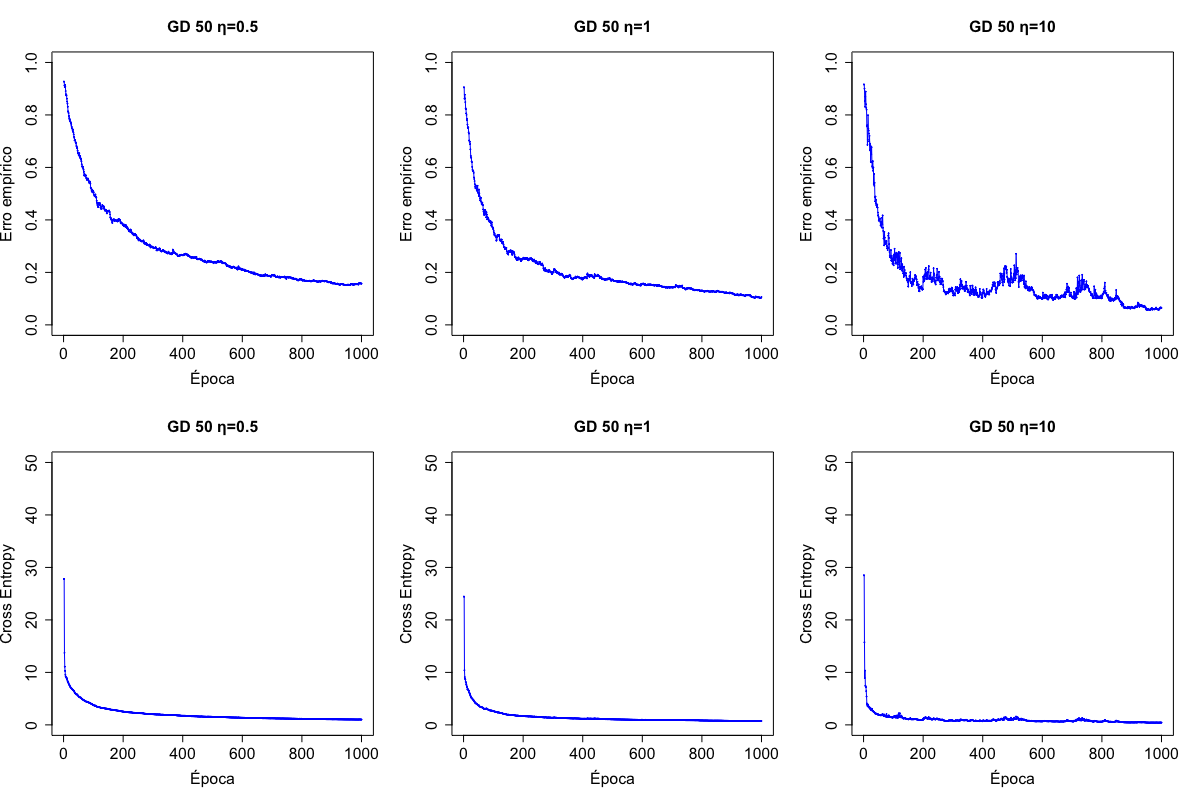
\includegraphics[width=\linewidth]{gd_50.png}
  \label{fig:gd_50}
  \caption{GD 50}
\end{figure}

\begin{figure}
  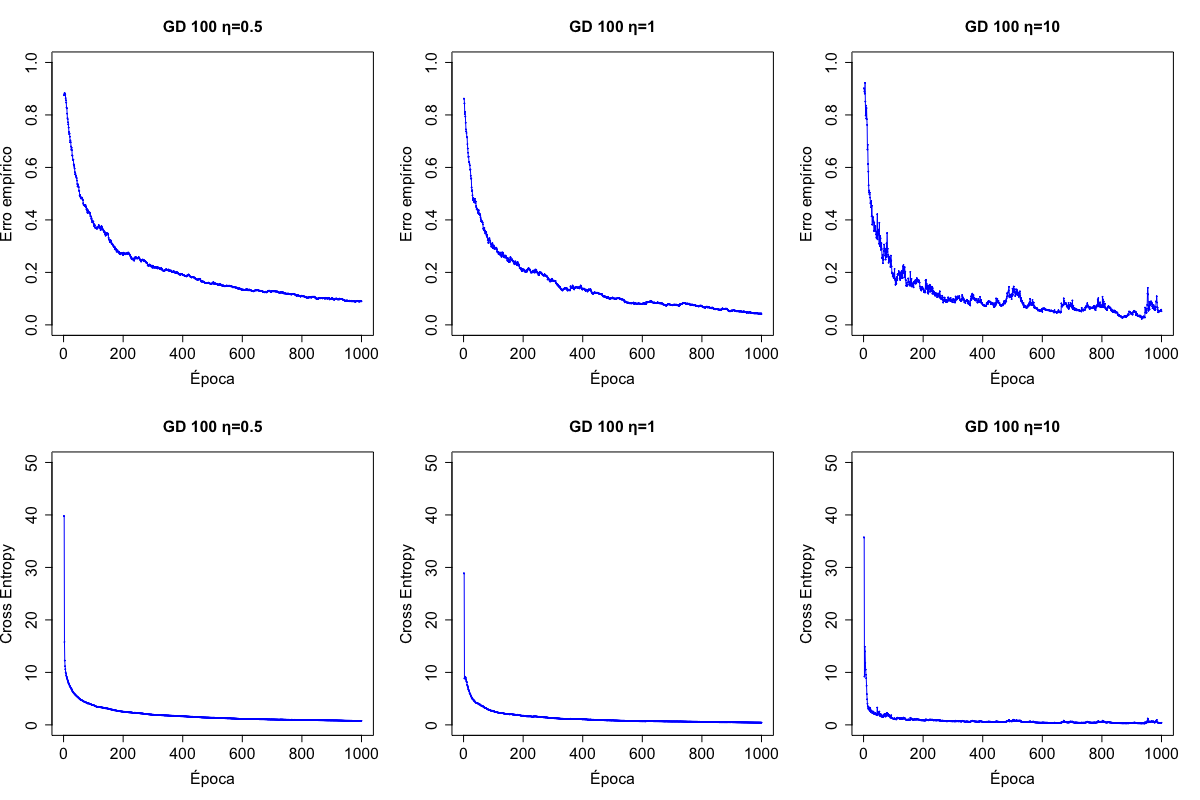
\includegraphics[width=\linewidth]{gd_100.png}
  \label{fig:gd_100}
  \caption{GD 100}
\end{figure}

\begin{figure}
  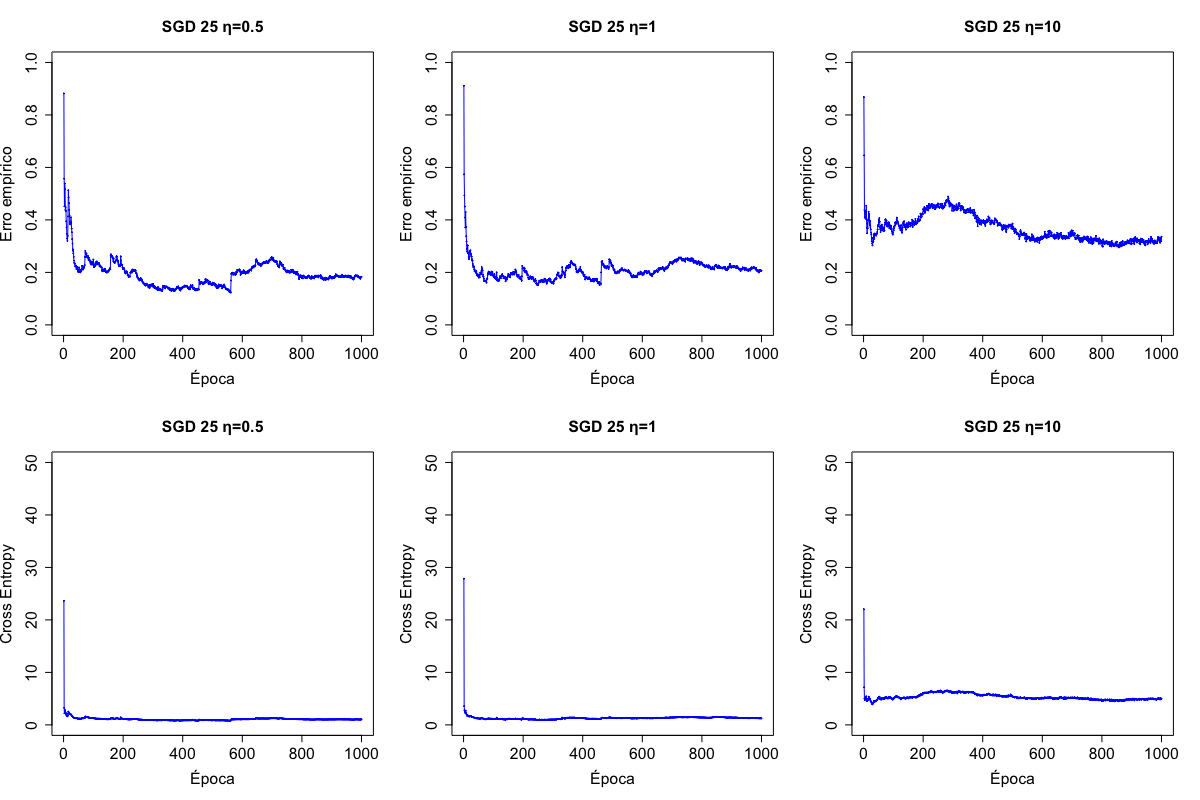
\includegraphics[width=\linewidth]{sgd_25.png}
  \label{fig:sgd_25}
  \caption{SGD 25}
\end{figure}

\begin{figure}
  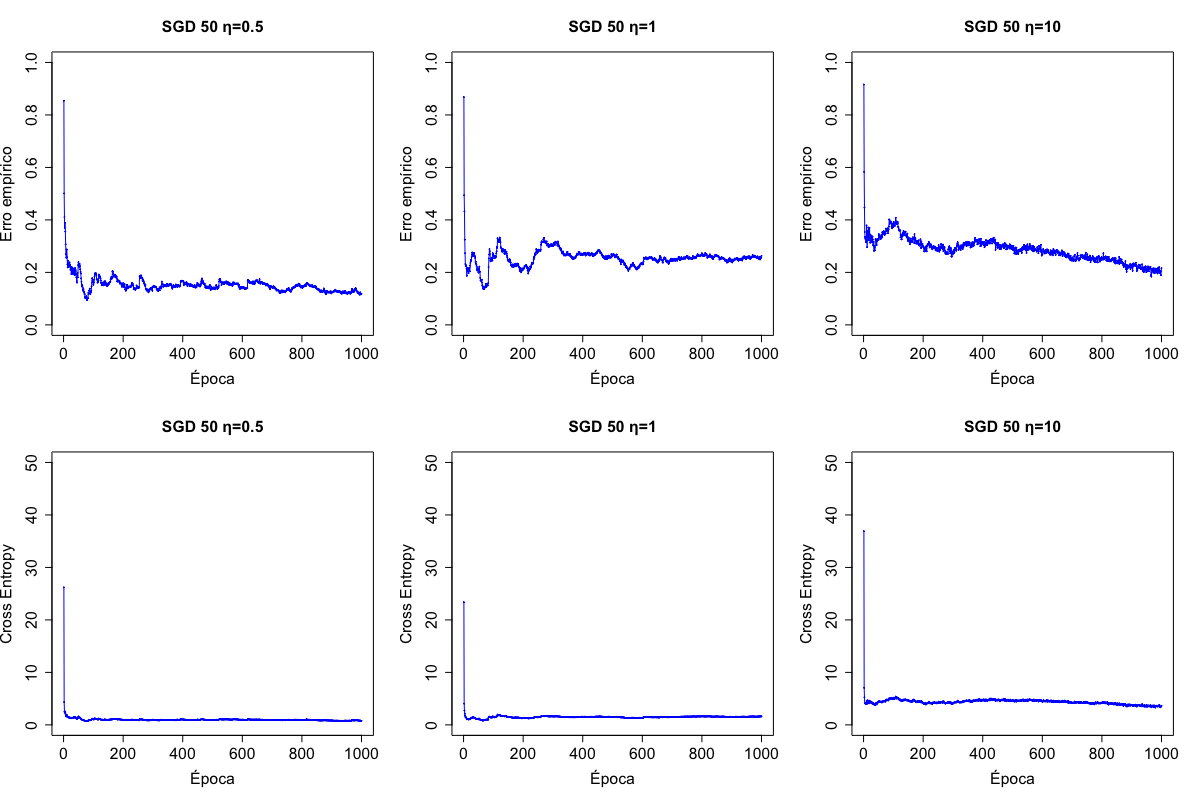
\includegraphics[width=\linewidth]{sgd_50.png}
  \label{fig:sgd_50}
  \caption{SGD 50}
\end{figure}

\begin{figure}
  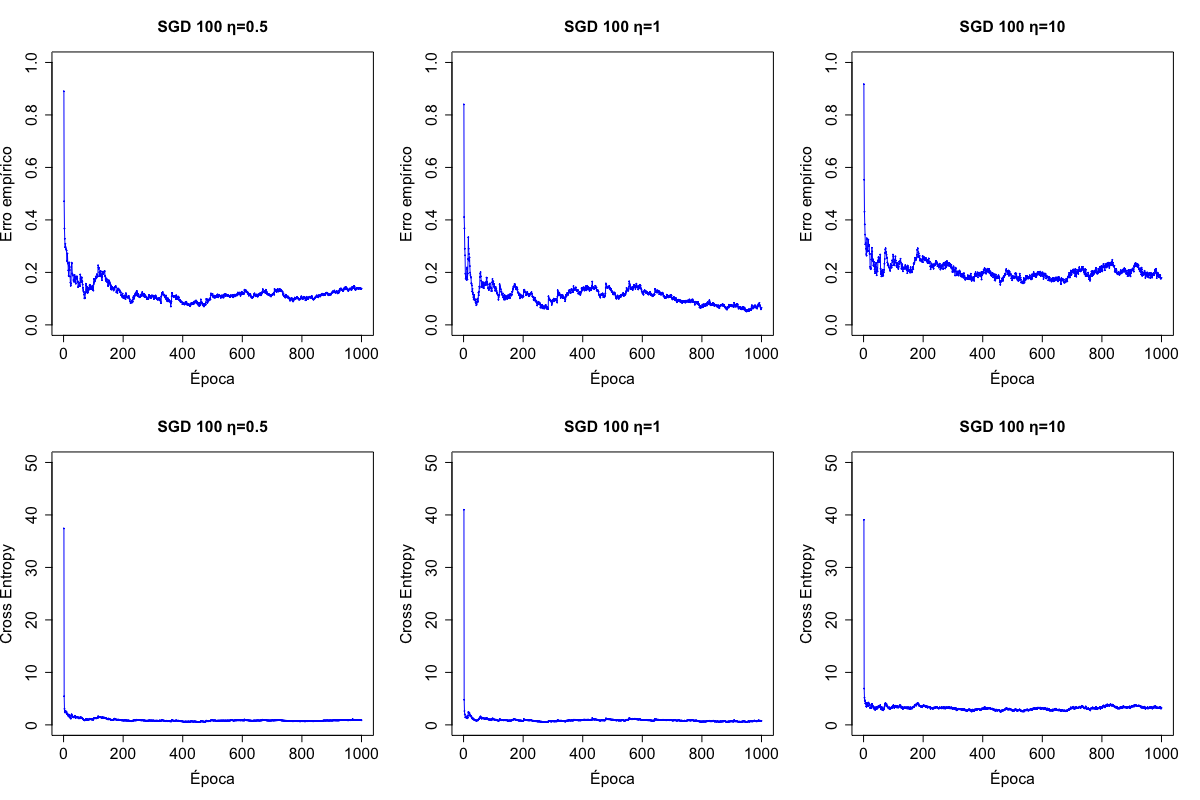
\includegraphics[width=\linewidth]{sgd_100.png}
  \label{fig:sgd_100}
  \caption{SGD 100}
\end{figure}

\begin{figure}
  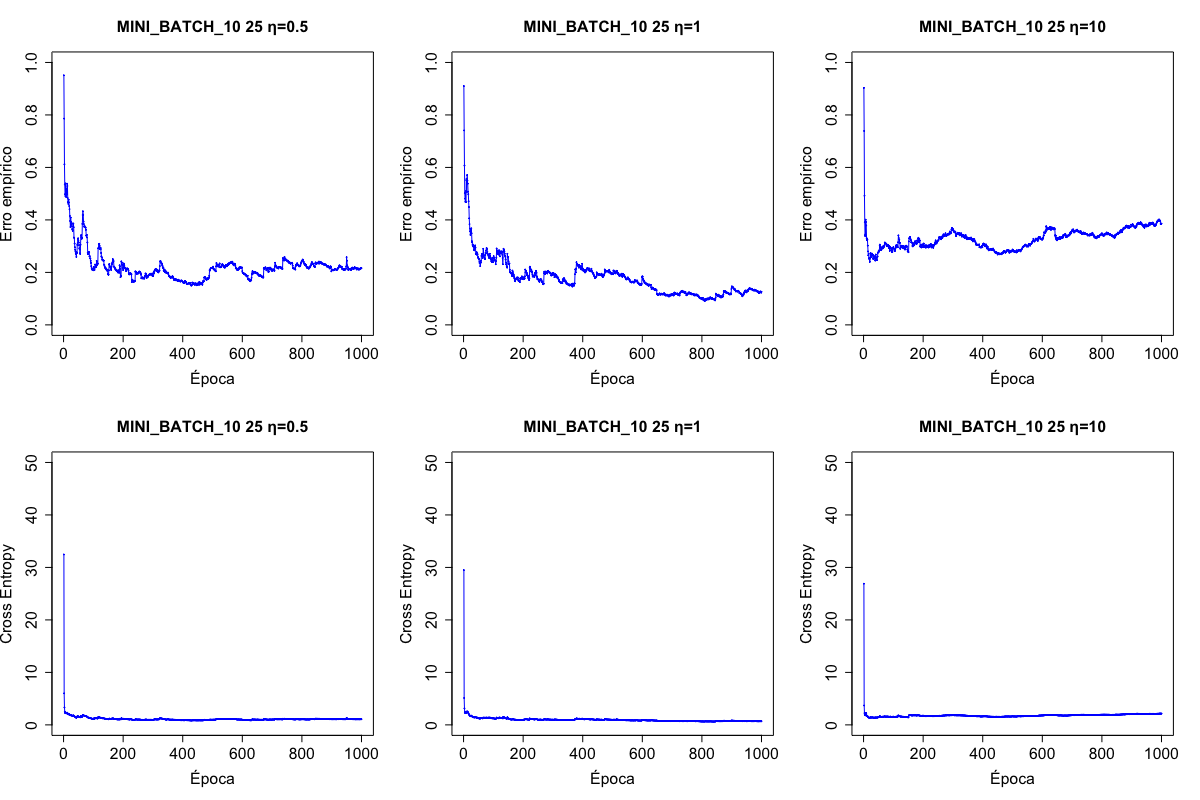
\includegraphics[width=\linewidth]{mini_batch_10_25.png}
  \label{fig:mini_batch_10_25}
  \caption{Mini Batch 10 (25)}
\end{figure}

\begin{figure}
  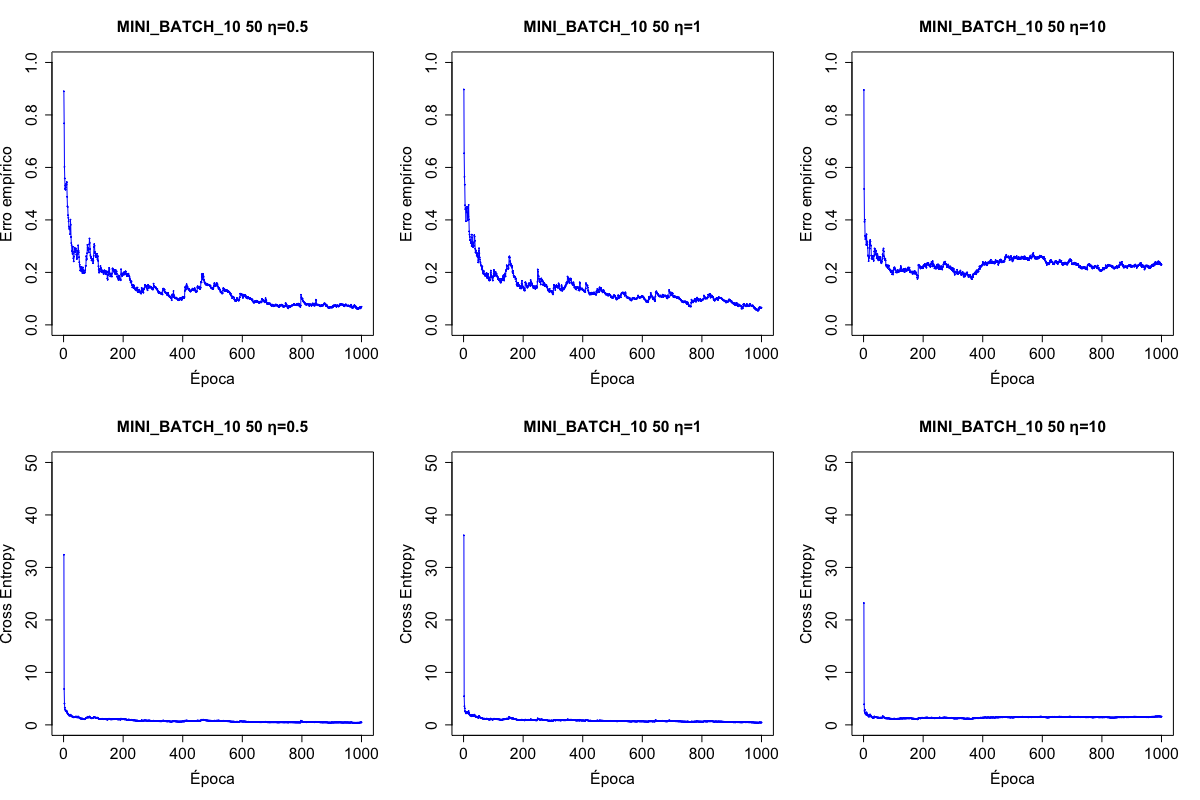
\includegraphics[width=\linewidth]{mini_batch_10_50.png}
  \label{fig:mini_batch_10_50}
  \caption{Mini Batch 10 (50)}
\end{figure}

\begin{figure}
  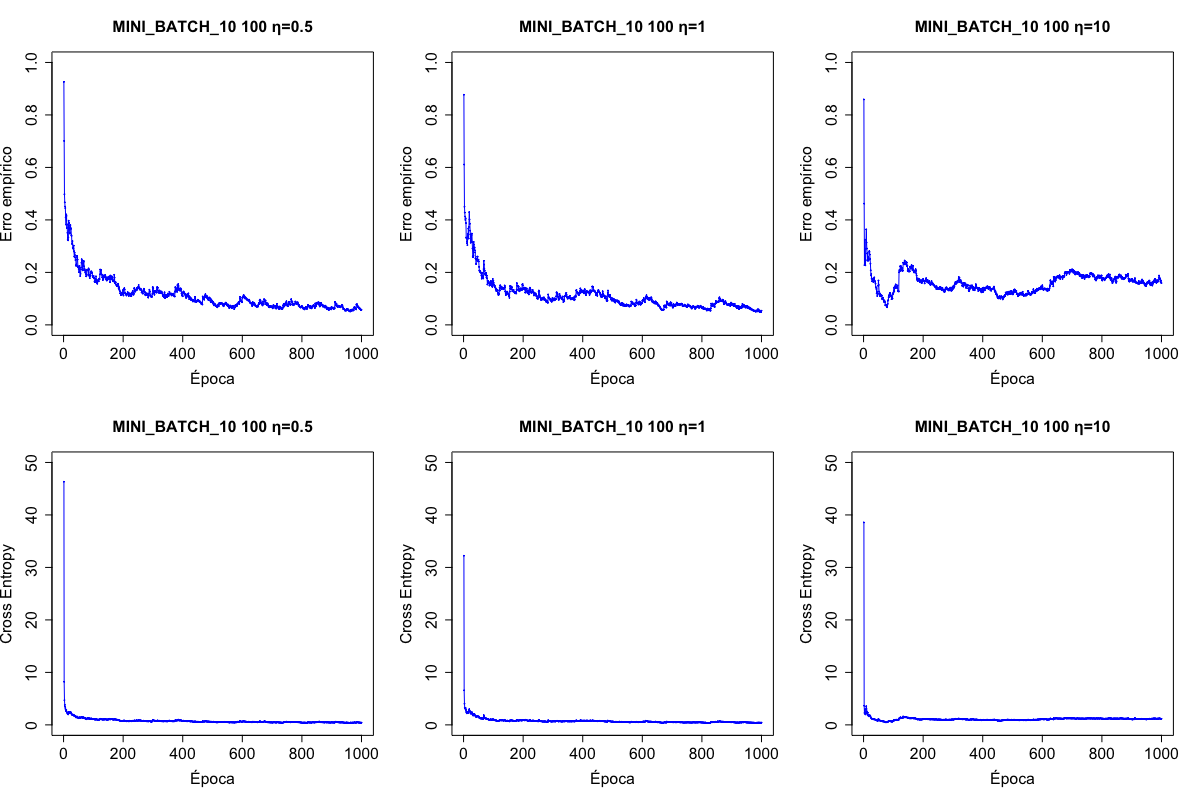
\includegraphics[width=\linewidth]{mini_batch_10_100.png}
  \label{fig:mini_batch_10_100}
  \caption{Mini Batch 10 (100)}
\end{figure}

\begin{figure}
  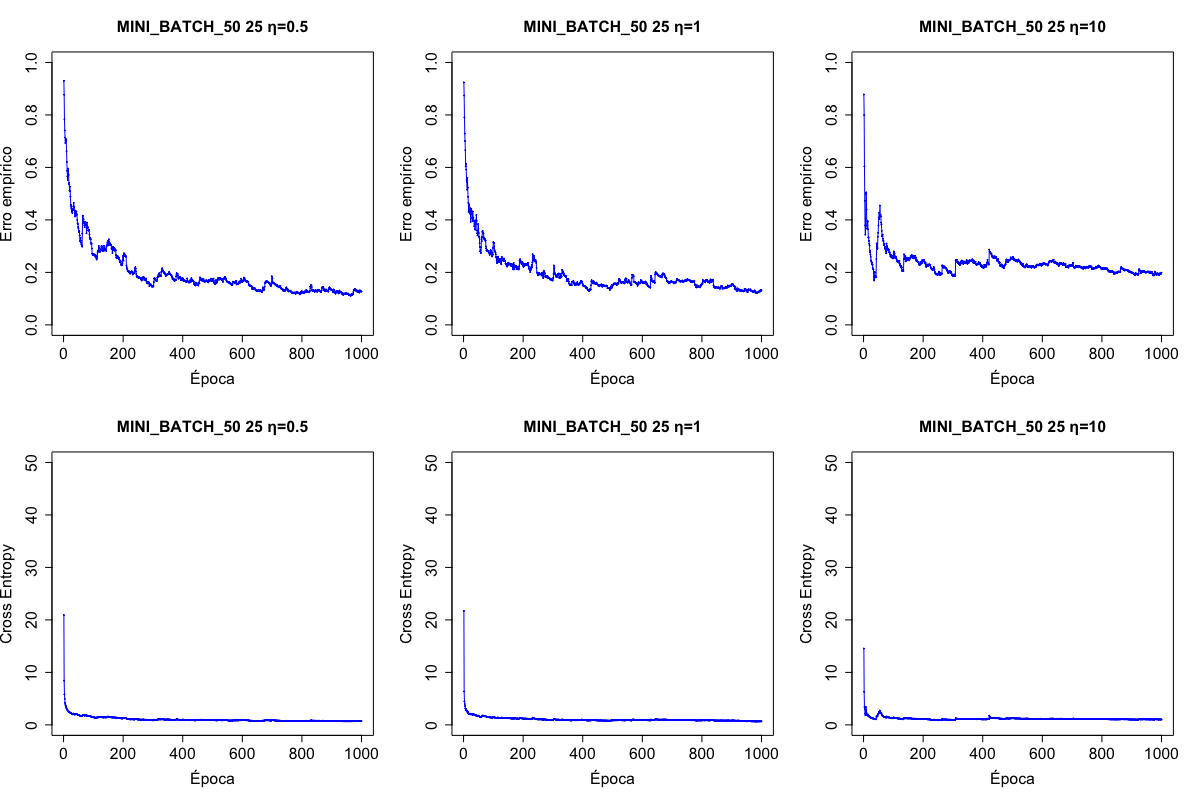
\includegraphics[width=\linewidth]{mini_batch_50_25.png}
  \label{fig:mini_batch_50_25}
  \caption{Mini Batch 50 (25)}
\end{figure}

\begin{figure}
  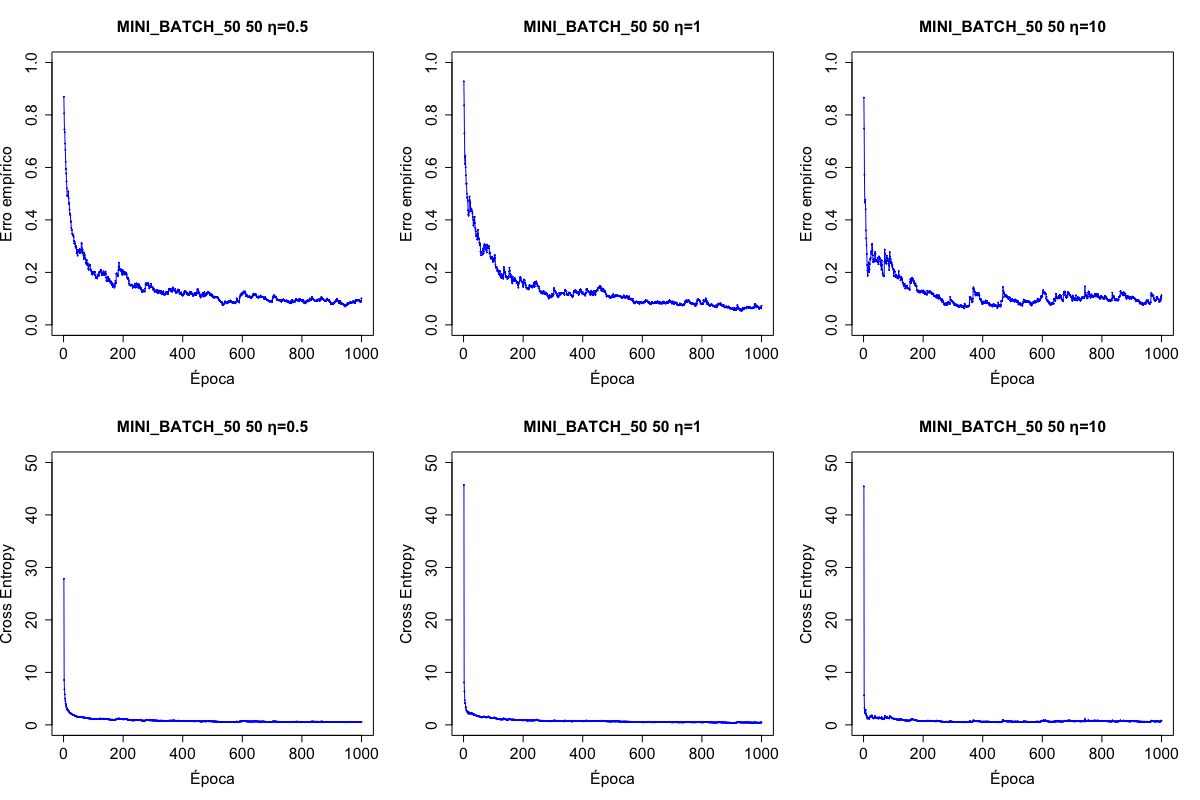
\includegraphics[width=\linewidth]{mini_batch_50_50.png}
  \label{fig:mini_batch_50_50}
  \caption{Mini Batch 50 (50)}
\end{figure}

\begin{figure}
  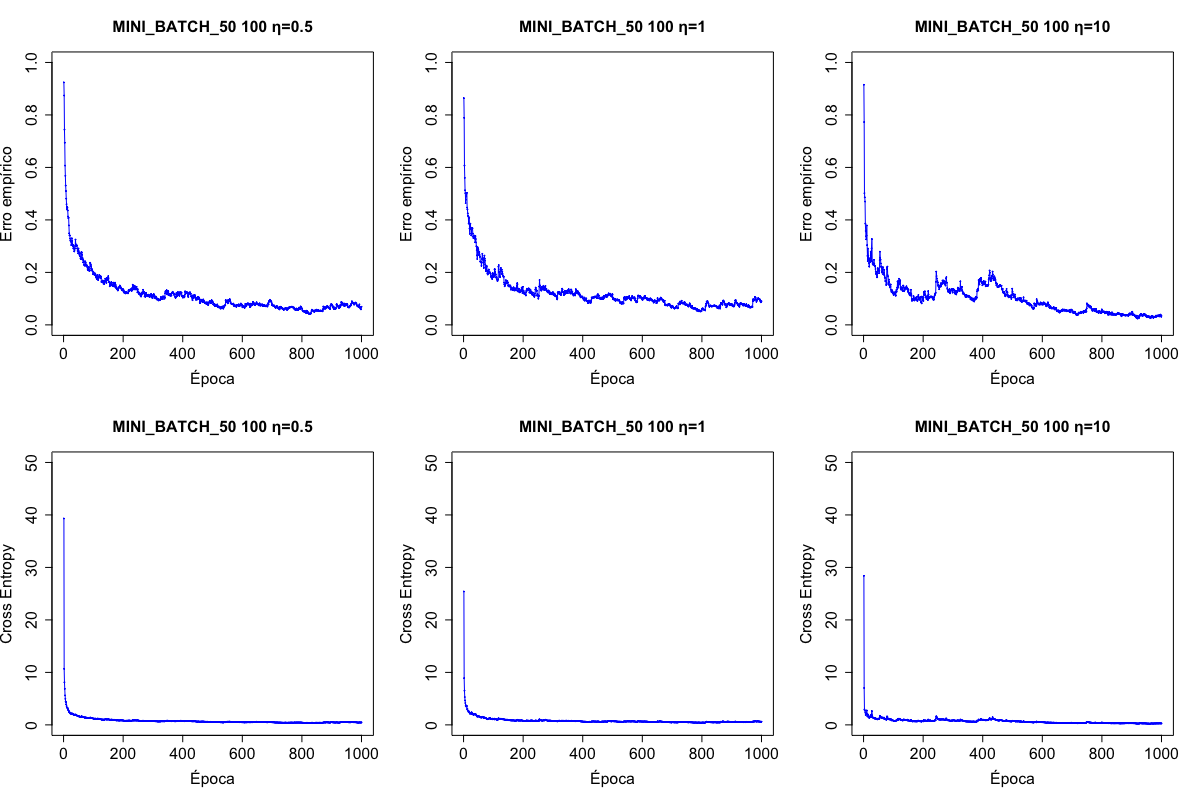
\includegraphics[width=\linewidth]{mini_batch_50_100.png}
  \label{fig:mini_batch_50_100}
  \caption{Mini Batch 50 (100)}
\end{figure}

\chapter{Conclusão}

Os experimentos realizados mostraram que diferentes estratégias de otimização se diferenciaram
na velocidade da redução da função de perda. É interessante notar que o erro empírico ficou
sempre em torno de 90\% antes do começo do treinamento da rede. Isso se deu porque, como os pesos
foram inicializados de forma aleatória e a rede prevê um valor de saída entre 0 e 9, ela
acerta em média 10\% dos casos sem nenhum treinamento.

Em todos os casos, a redução da função de perda aconteceu de forma dramática no começo e ficou
bem mais lenta após a passagem de algumas épocas.

O aumento da taxa de aprendizado $ \eta $ em todos os casos contribuiu para um aumento do ruído
no processo de minimização da função de perda, no entanto, também é possível notar, principalmente
nos experimentos que utilizaram o modelo GD e Mini Batch 50, que o aumento da taxa de aprendizado
acelerou consideravelmente o processo de convergência.

A trajetória de atualização dos pesos no modelo SGD se mostrou muito mais errática do que nos modelos
Mini Batch, que, por sua vez, se mostraram mais erráticos do que o modelo GD. No entanto, o
Mini Batch 50 já mostrou um desempenho bastante similar ao GD, com o bônus de realizar a convergência
mais rapidamente.

O aumento do número de neurônios na camada oculta mostrou que mais neurônios permitiram que o erro empírico
convergisse para um valor menor. Isso aconteceu porque o aumento da capacidade da rede permitiu a modelagem
de funções mais complexas. No entanto, a maior redução do erro empírico nos modelos que utilizaram 100 
neurônios ocultos não significa que estas redes tenham um erro esperado menor (devido ao Overfitting).

Por fim, os modelos que tiveram o melhor desempenho foram o GD 100 com $ \eta = 10 $ chegando ao erro
empírico de 2.3\% após 1000 épocas e o Mini Batch 50 com 100 neurônios ocultos e $ eta = 10 $ que reduziu
o erro empírico para 2.4\% após 1000 iterações. No entanto, na média, o Mini Batch 50 teve um desempenho
melhor do que o GD, convergindo mais rápido para valores baixos da Cross Entropy.

\end{document}
